\textcolor{ubuntu_orange}{Konta sieciowe} to specjalny program w Ubuntu, pozwalający sprząc system bezpośrednio z różnymi dostawcami usług sieciowych. Przykładowo, po dodaniu konta Google można łączyć się z czatem Google za pomocą wbudowanego programu Empathy, czy synchronizować zdjęcia z usługą Picasa za pośrednictwem programu Shotwell. Na podobnej zasadzie działa połączenie z kontem Facebooka, Flickr czy Twittera. Użycie \textcolor{ubuntu_orange}{Kont sieciowych} pozwala skorzystać z dwustopniowego uwierzytelnienia, nawet w programach, które w innych warunkach tego nie potrafią.

\begin{center}
	\begin{tikzpicture}
	\node[anchor=south west,inner sep=0] (image) at (0,0) {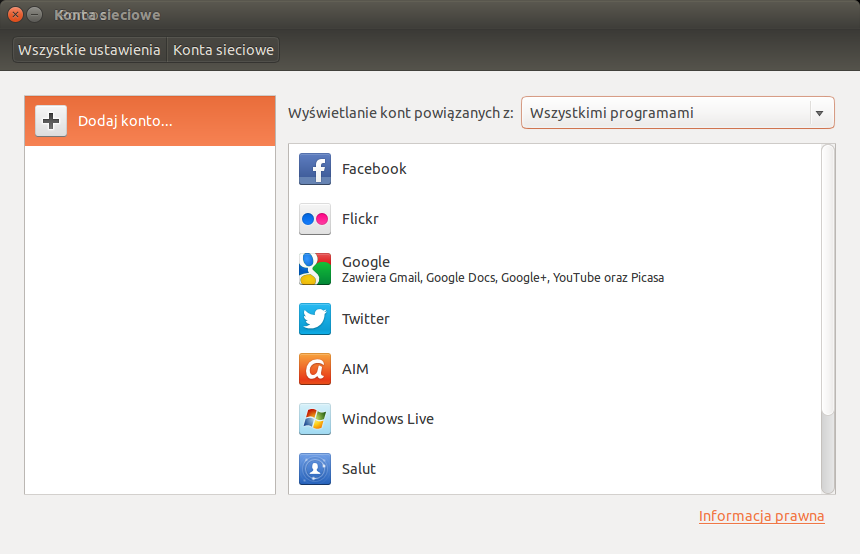
\includegraphics[width=\linewidth]{images/programy_kontaOnline1.png}};
	\begin{scope}[x={(image.south east)},y={(image.north west)}]
		\draw[ubuntu_orange,line width=3pt,rounded corners] (0.02,0.72) rectangle (0.33,0.83);
		\draw[ubuntu_orange,line width=3pt,fill=white,fill opacity=0.75] (0.15,0.55) circle [radius=0.30cm]
			node[text=black]{\Large \textbf 1};
		\draw[ubuntu_orange,dashed,line width=3pt] (0.15,0.57) -- (0.15,0.70);
    \end{scope}
\end{tikzpicture}
\end{center}

Aby dodać konto do systemu, wyszukaj w Dashu \textcolor{ubuntu_orange}{Konta sieciowe} i uruchom program. W otwartym oknie kliknij \textcolor{ubuntu_orange}{+ Dodaj konto} \circled 1 w lewym panelu, a następnie z prawego wybierz interesującego cię dostawcę. Zostaniesz teraz poproszony o uwierzytelnienie usługi w systemie.

Możesz zsynchronizować więcej niż jedną usługę. Program \textcolor{ubuntu_orange}{Konta sieciowe} pozwala ponadto zarządzać tym, jakie programy do jakich usług mają dostęp. 
